% Exemplos 1--4 do cap. 5: transcrição cientificamente ancorada
% dos fontes mb-uso/secoes/exemplo_01.tex ... exemplo_04.tex.
% Todos os gráficos são arquivos vetoriais originais em mb-uso/figuras/.

\begin{frame}[plain]
\vspace{1.8cm}{\LARGE\color{navy}Exemplos de uso\par}\vspace{.3cm}\textcolor{navy!40}{\rule{.76\linewidth}{.65pt}}\par
\vspace{.20cm}Resultados produzidos pelo MoeaBench e interpretação dos experimentos
\end{frame}

\begin{frame}[fragile]{Exemplo 1 — Em que região da frente o algoritmo chegou?}
\begin{columns}[T,onlytextwidth]
\begin{column}{.40\textwidth}
\textbf{DTLZ2:} 3 objetivos, NSGA-III com 50 indivíduos, 50 gerações.
\begin{lstlisting}[style=python,basicstyle=\ttfamily\fontsize{8}{10}\selectfont]
exp1 = mb.experiment()
exp1.mop = mb.mops.DTLZ2(M=3)
exp1.moea = mb.moeas.NSGA3(
    population=50,
    generations=50)
exp1.run()

print(len(exp1.non_dominated()))
mb.view.topology(exp1)
\end{lstlisting}
\textbf{Resultado:} 50 soluções não dominadas na população final.
\end{column}
\begin{column}{.58\textwidth}
\centering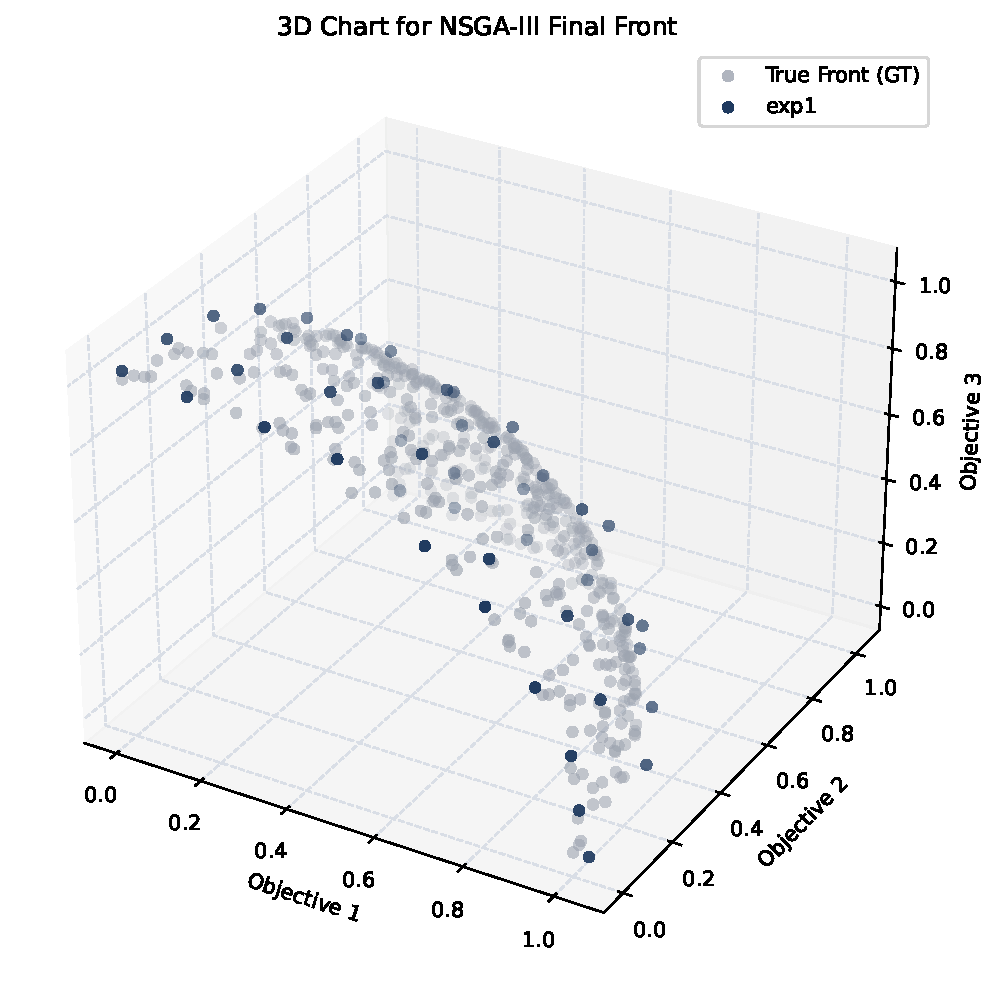
\includegraphics[width=\linewidth,height=.57\textheight,keepaspectratio]{figures/example_01_01_topology.pdf}
\par\smallskip {\scriptsize Soluções obtidas (azul) comparadas à frente esférica de referência do DTLZ2 (cinza).}
\end{column}
\end{columns}

\end{frame}

\begin{frame}[fragile]{Exemplo 1 — Como a qualidade evoluiu durante a busca?}
\begin{columns}[T,onlytextwidth]
\begin{column}{.67\textwidth}
\centering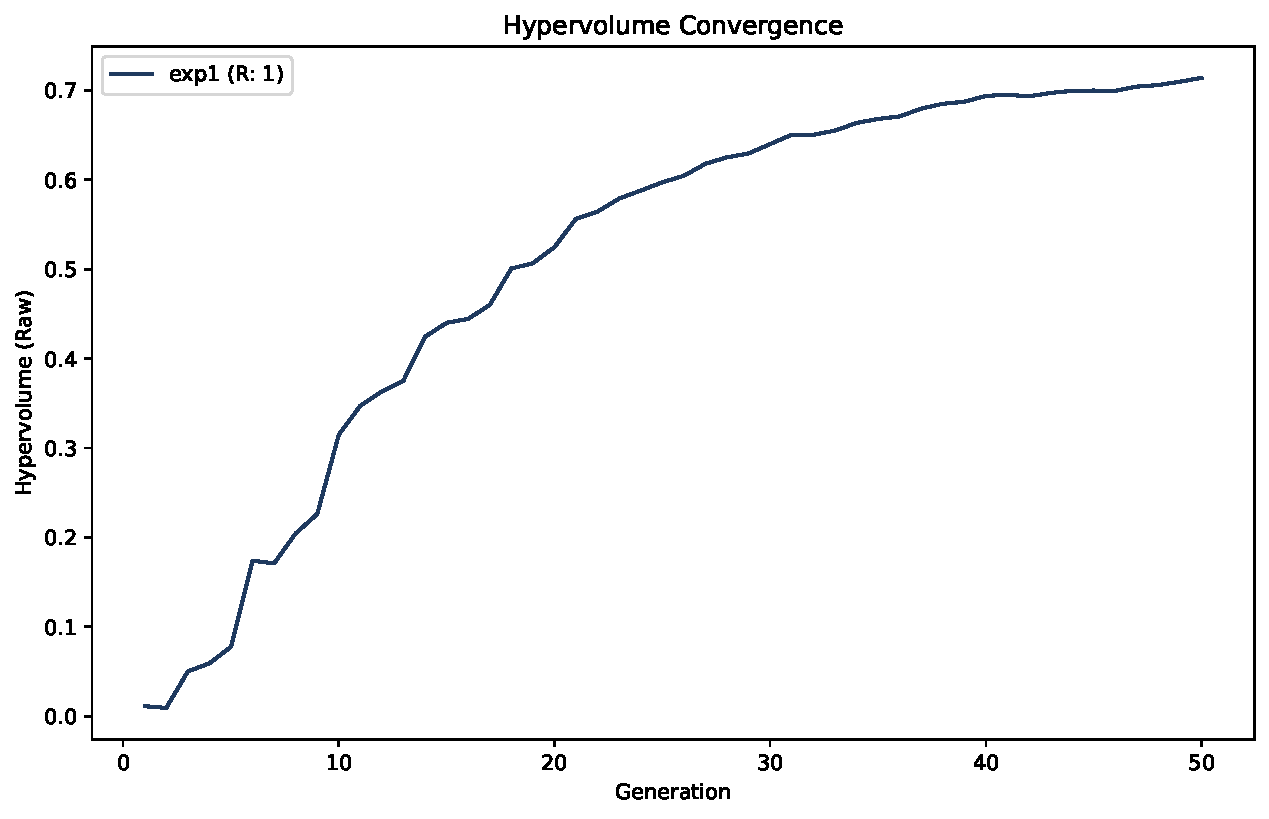
\includegraphics[width=\linewidth,height=.60\textheight,keepaspectratio]{figures/example_01_02_history.pdf}
\end{column}
\begin{column}{.31\textwidth}
\begin{lstlisting}[style=python,basicstyle=\ttfamily\fontsize{7.7}{9.5}\selectfont]
hv = mb.metrics.hv(exp1)
print(hv.gen(0), hv.last)
mb.view.history(hv)
\end{lstlisting}
\textbf{HV inicial:} 0,011207

\textbf{HV final:} 0,713990

O volume dominado cresce substancialmente; nas gerações finais, a curva tende a um patamar.
\end{column}
\end{columns}
\vspace{.03cm}
\textbf{Leitura conjunta:} a topologia mostra \emph{onde} ficaram as soluções; o histórico mostra \emph{quanto} a busca progrediu.
\end{frame}

\begin{frame}[fragile]{Exemplo 2 — Duas frentes finais: NSGA-III e SPEA2}
\begin{columns}[T,onlytextwidth]
\begin{column}{.36\textwidth}
Mesmo MOP: \textbf{DTLZ2 com 3 objetivos}; ambos com 50 indivíduos e 50 gerações.
\begin{lstlisting}[style=python,basicstyle=\ttfamily\fontsize{8}{10}\selectfont]
# Experimentos previamente
# configurados com NSGA-III
# e SPEA2, respectivamente:
exp1.run()
exp2.run()

mb.view.topology(exp1, exp2)
\end{lstlisting}
A figura compara a ocupação da frente de referência pelas duas populações finais.
\end{column}
\begin{column}{.62\textwidth}
\centering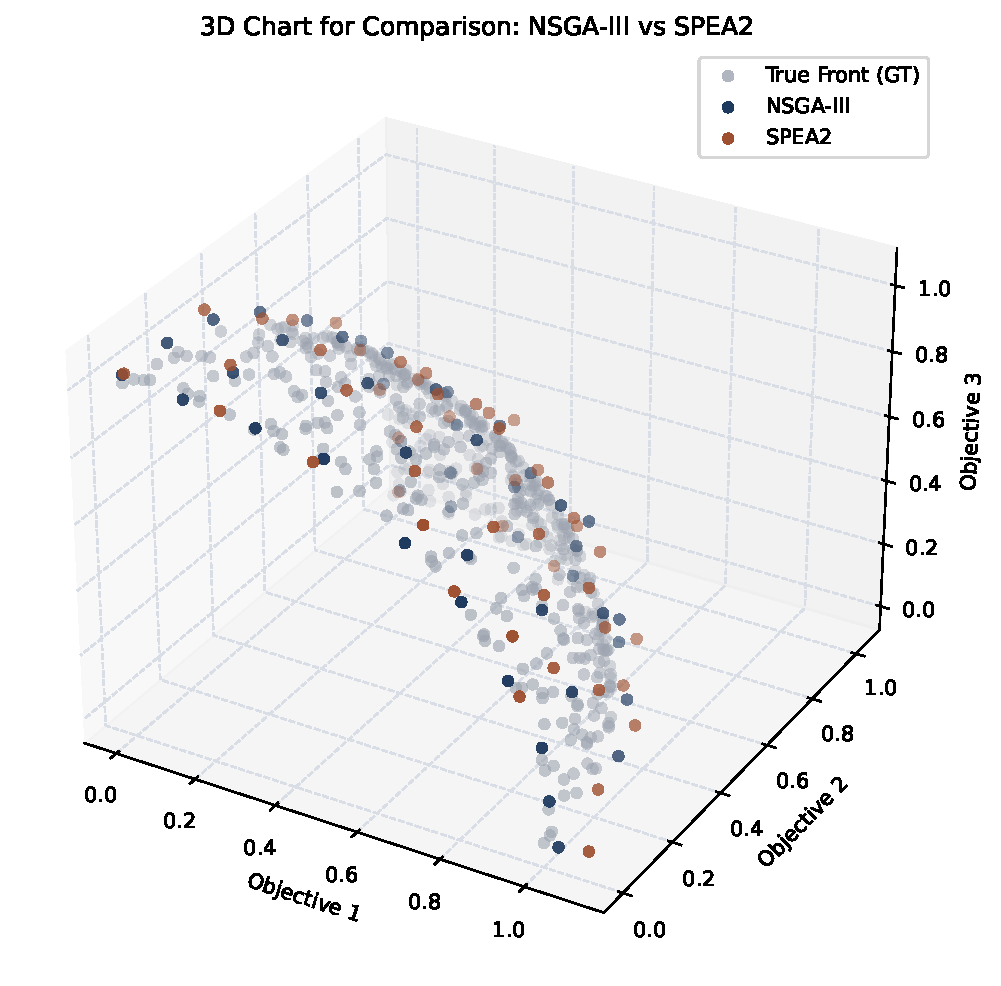
\includegraphics[width=\linewidth,height=.61\textheight,keepaspectratio]{figures/example_02_01_topology.pdf}
\end{column}
\end{columns}

\end{frame}

\begin{frame}[fragile]{Exemplo 2 — Resultado final próximo, trajetórias diferentes}
\begin{columns}[T,onlytextwidth]
\begin{column}{.66\textwidth}
\centering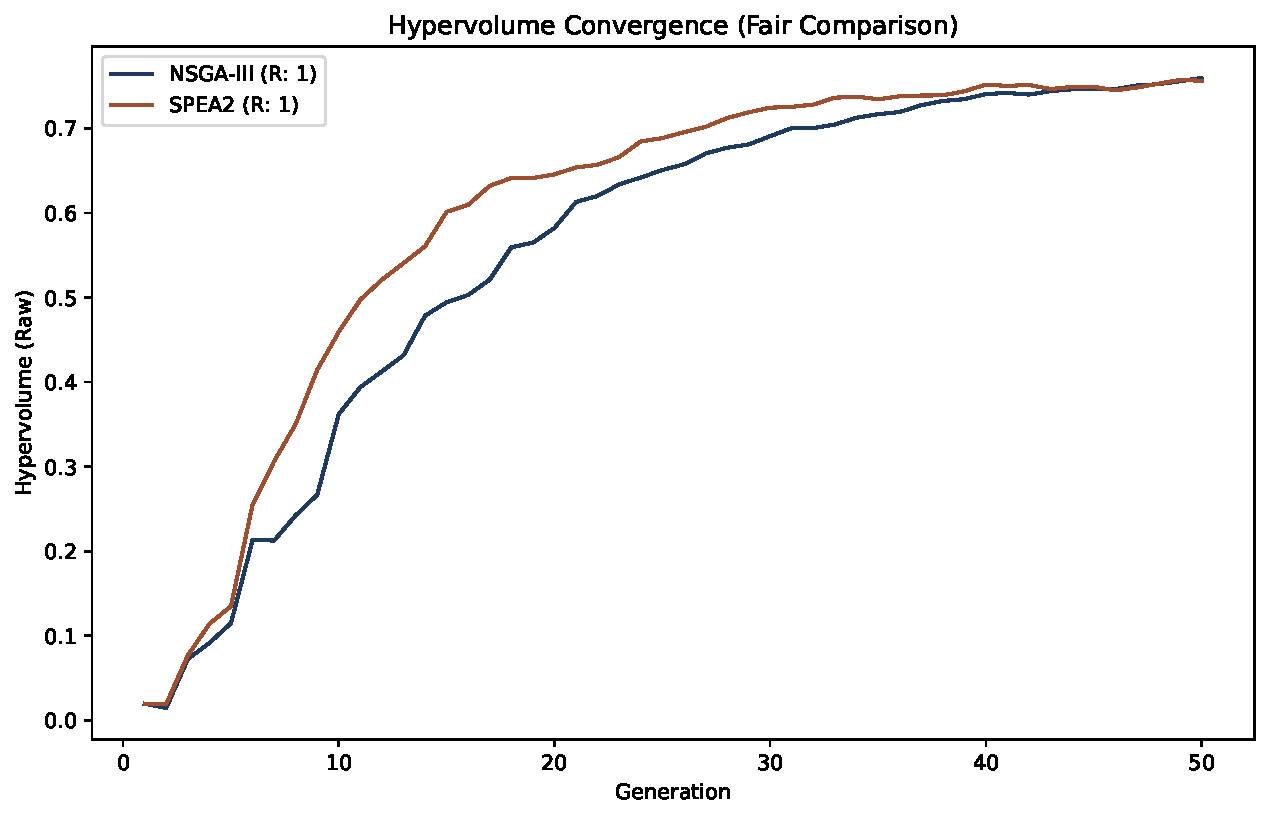
\includegraphics[width=\linewidth,height=.58\textheight,keepaspectratio]{figures/example_02_02_history.pdf}
\end{column}
\begin{column}{.32\textwidth}
\begin{lstlisting}[style=python,basicstyle=\ttfamily\fontsize{7.4}{9.2}\selectfont]
ref = [exp1, exp2]
hv1 = mb.metrics.hv(
    exp1, ref=ref)
hv2 = mb.metrics.hv(
    exp2, ref=ref)
mb.view.history(hv1, hv2)
\end{lstlisting}
\textbf{HV final:}

NSGA-III: \textbf{0,759872}

SPEA2: \textbf{0,756493}
\end{column}
\end{columns}
\vspace{.01cm}
\textbf{Leitura:} o SPEA2 avançou mais rapidamente durante parte da busca, mas o NSGA-III terminou ligeiramente à frente; \texttt{ref} comum torna o HV comparável.
\end{frame}

\begin{frame}[fragile]{Exemplo 3 — Quais soluções comparar e em que geração?}
\begin{columns}[T,onlytextwidth]
\begin{column}{.41\textwidth}
\textbf{DTLZ2, NSGA-III:} 100 indivíduos, 100 gerações.
\begin{lstlisting}[style=python,basicstyle=\ttfamily\fontsize{7.7}{9.5}\selectfont]
exp1.run()
print(len(exp1.non_dominated()),
      len(exp1.dominated()))
mb.view.topology(
    exp1.front(),
    exp1.non_front())
mb.view.topology(
    exp1.front(5), exp1)
\end{lstlisting}
\textbf{Resultado final:} 100 não dominadas; nenhuma dominada na população final.
\end{column}
\begin{column}{.57\textwidth}
\centering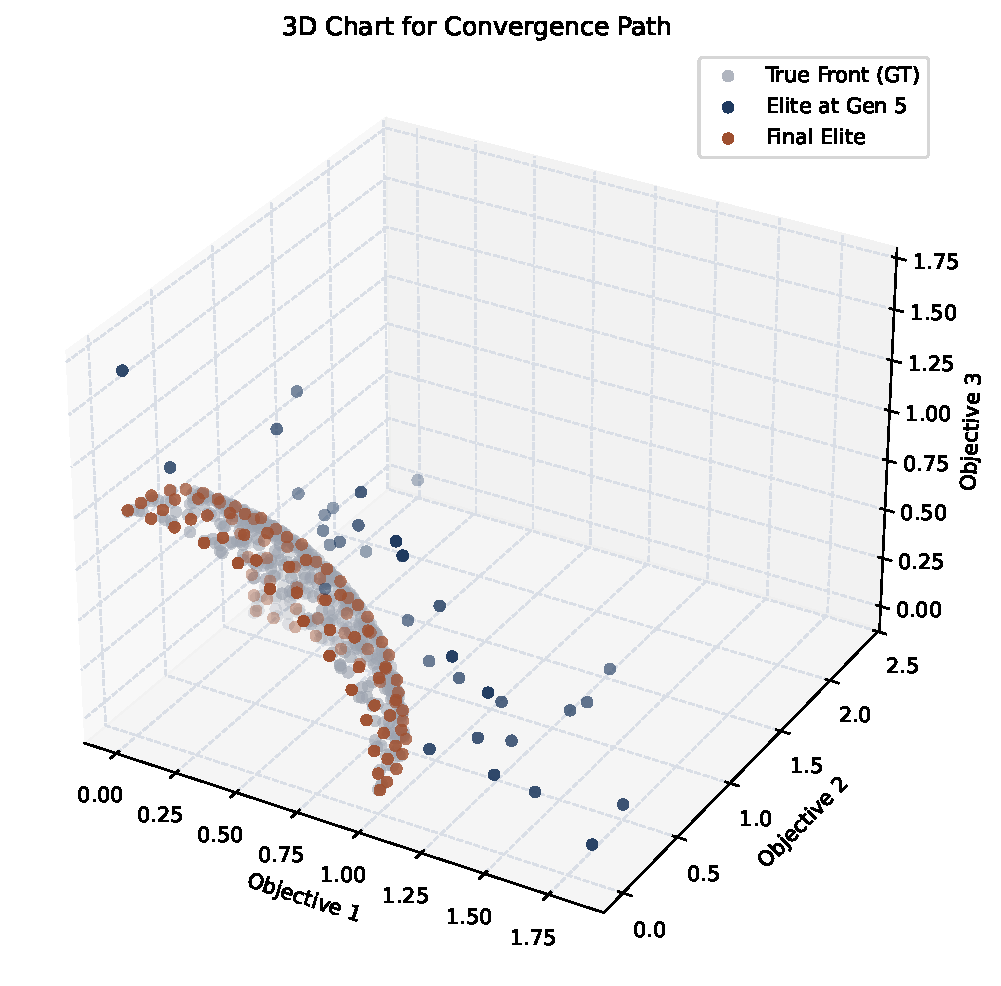
\includegraphics[width=\linewidth,height=.60\textheight,keepaspectratio]{figures/example_03_02_topology.pdf}
\end{column}
\end{columns}
\vspace{.02cm}
\textbf{Leitura:} na geração de índice 5, há soluções distantes da frente teórica; na população final, elas se concentram junto à superfície esférica.
\end{frame}

\begin{frame}[fragile]{Exemplo 4 — Uma boa execução não basta para avaliar estabilidade}
\begin{columns}[T,onlytextwidth]
\begin{column}{.61\textwidth}
\centering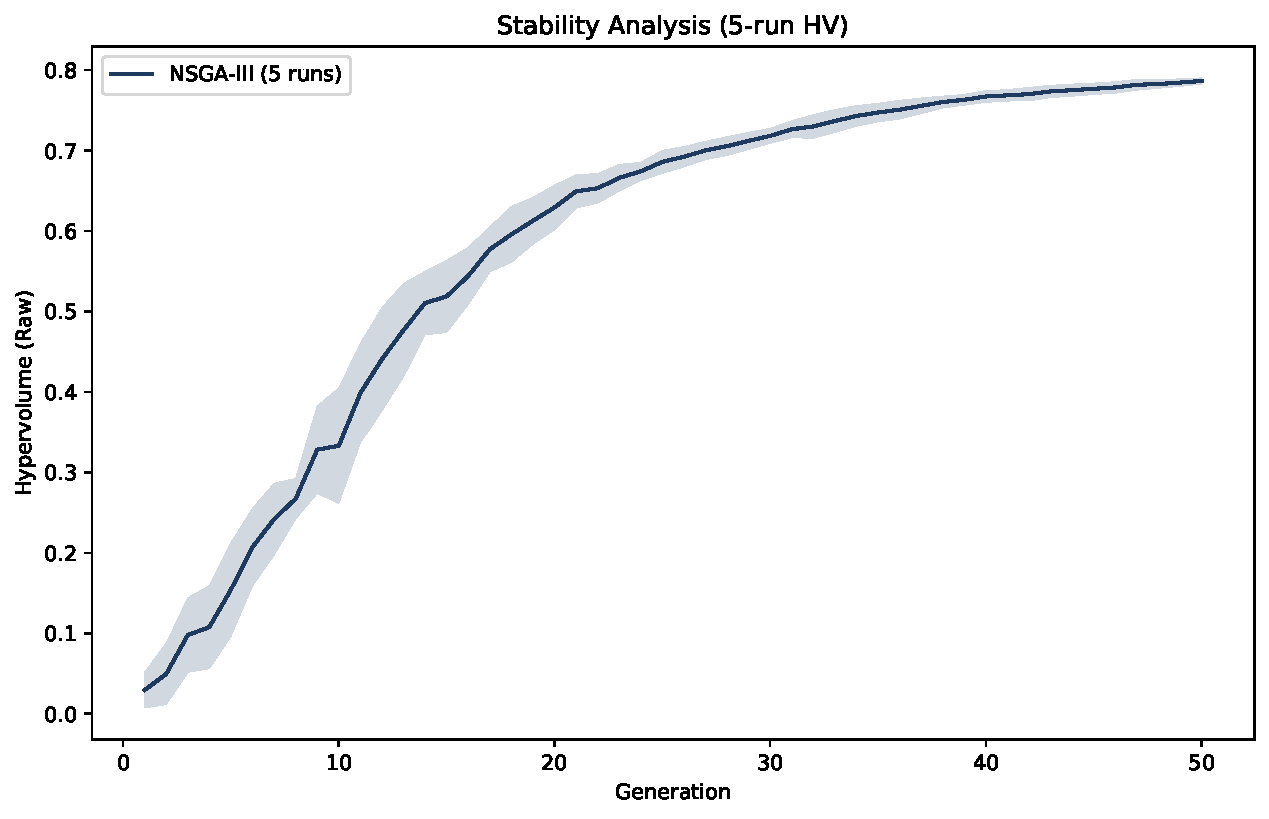
\includegraphics[width=\linewidth,height=.58\textheight,keepaspectratio]{figures/example_04_01_history.pdf}
\end{column}
\begin{column}{.37\textwidth}
\begin{lstlisting}[style=python,basicstyle=\ttfamily\fontsize{7.4}{9.2}\selectfont]
exp1.run(repeat=5)
hv = mb.metrics.hv(exp1)
print(hv.last, hv.std())
mb.view.history(hv)
\end{lstlisting}
\textbf{Média final do HV:} 0,786496

\textbf{Desvio-padrão:} 0,003830
\end{column}
\end{columns}
\vspace{.02cm}
\textbf{Leitura:} a dispersão do HV diminui ao longo da busca. Um desvio-padrão pequeno não prova que as frentes ocupam as mesmas regiões.
\end{frame}

\begin{frame}[fragile]{Exemplo 4 — Estabilidade do HV não significa frentes idênticas}
\begin{columns}[T,onlytextwidth]
\begin{column}{.62\textwidth}
\centering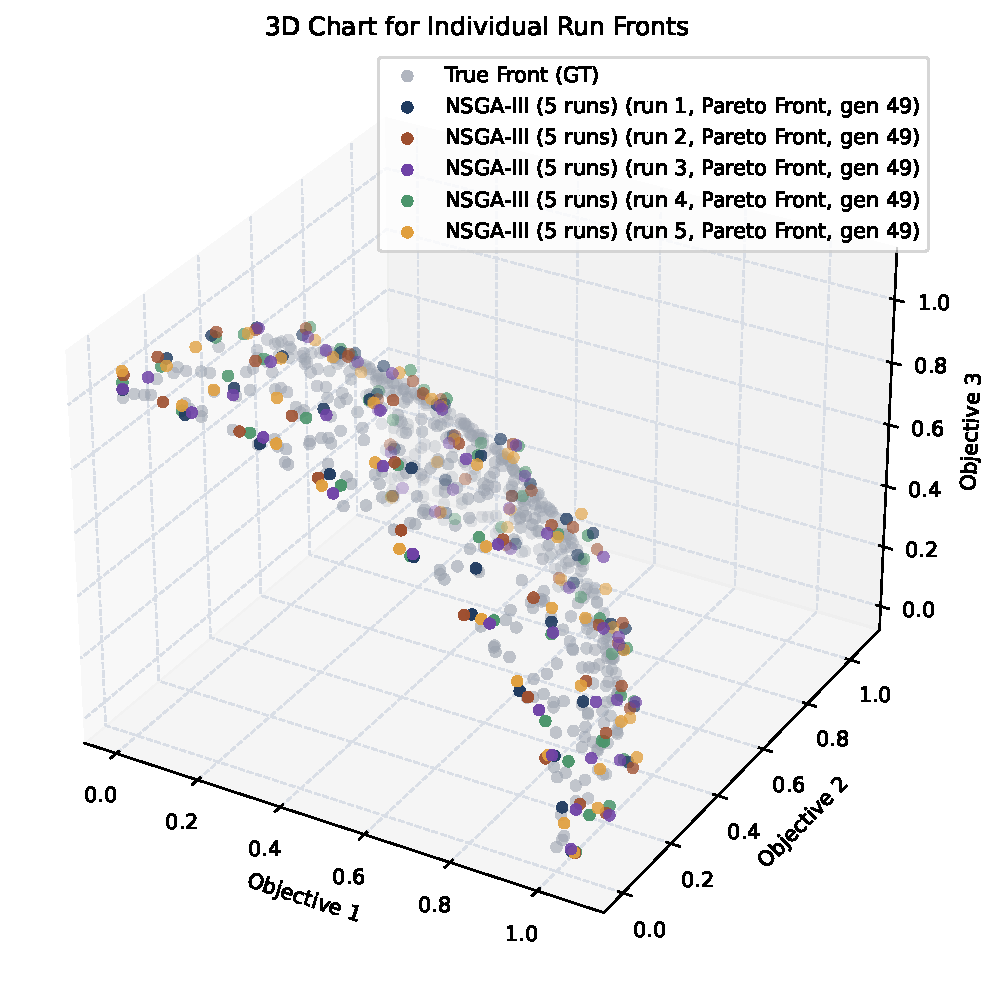
\includegraphics[width=\linewidth,height=.61\textheight,keepaspectratio]{figures/example_04_05_topology.pdf}
\end{column}
\begin{column}{.36\textwidth}
\begin{lstlisting}[style=python,basicstyle=\ttfamily\fontsize{7.7}{9.5}\selectfont]
ratio = mb.metrics.front_ratio(
    exp1)
print(ratio.last)
fronts = exp1.all_fronts()
mb.view.topology(*fronts)
\end{lstlisting}
\textbf{Resultado:} \texttt{front\_ratio}=1,0000 ao final de cada rodada.

Ao reunir as cinco populações: \textbf{250} soluções, das quais \textbf{185} globalmente não dominadas.
\end{column}
\end{columns}
\vspace{.01cm}
\textbf{Leitura:} uma solução não dominada em uma execução pode ser dominada por soluções de outra. A topologia complementa a estabilidade medida pelo HV.
\end{frame}
